\chapter{Results and Discussion}\label{C:results}\label{C:evaluation}

The following section reports on the outcome of several experiments that explore the use of our framework on a realistic benchmark suite. The key factors of interest are -- the time taken, number of comparisons, the types of redundant tests identified and the overall cost of performance (time) vs precision (tests identified \& types identified). \todo{Link back to req?}

There are two points that the reader needs to be aware of. Firstly, in the significant tables below, a `+' represents that significant increase, `-' significant decrease and `=' represents no significant difference. Secondly, the graphs are displayed using a logarithm scale.

\section{Method}

The experiment method is key to producing believable and reproducible results. Before the experiment could be conducted, the data for each benchmark had to be retrieved. This involved setting the benchmark up locally and then executing the tests with the AspectJ class loader. The data was then run on a grid computing system. After the results had been returned, a Wilcoxon signed rank test \cite{wilcoxon1945individual} was used to determine whether the results were significantly different or not. The significant level used was 95\% with a null hypothesis of the two samples median being equal. Overall, seven different settings were run per benchmark with each setting being run 30 times.

The goals of this paper as mentioned in Section \ref{C:intro} are the creation of a framework to identify redundant test cases and experimenting with different techniques on realistic benchmarks. The rest of this chapter explores the experiments conducted to give guidance to the users of the tool.

\section{Environmental Methodologies}
\label{enviro}
As previously discussed in Section \ref{performanceEvalBG} there are a variety of challenges that present themselves when using Java to evaluate performance. These challenges are discussed throughout the following section.

\subsection{Grid Computing}
A grid computing system was used to execute the data analysis, with a total of 150 jobs queued on the grid at a single time. When using a grid system it is important to ensure that all the machines used are the same for every experiment. The grid allowed for particular types of machines to be specified -- 8gb ddr3 ram, Linux 4.0.5 64 bit system and an Intel Core i7-3770 CPU running @ 3.40GHz.

\subsection{Measuring Time}
The time taken is an important variable in evaluating the performance of a tool. In Java, this can be achieved by accessing a system method that returns the total time in milliseconds from 1970 00:00:00 UTC to the current time. Taking this time before the analysis, and subtracting from the time after the analysis gives the total time taken. This notation of time is defined as wall clock time. Utilising a grid system presents difficulties with using the wall clock time to measure the time taken. 

As mentioned in Section \ref{C:related}, when a job is run on the grid system, there is potential for the machine to be paused. If wall time were to be used, the time that the process is paused would also be included. To resolve this issue, the notation of CPU time was used. The CPU time is the measure of time in nanoseconds that the computer program spent on the CPU. Another concern is if a user logs in during analysis, the tool's RAM could potentially be moved into virtual memory. This is dependent on the amount of RAM that the user needs. When the user logs out, the tool will restart and any information lost will need to be recalculated by the tool. Both these issues were limited by running the tests overnight when users were unlikely to log in.

When measuring the time taken to analyse, the start up cost was not taken into account. Running up to 150 jobs meant that a large number of applications would be attempting to access a single data file at a single time. This stress on the system introduces a large amount of non-deterministic behaviour. Removing the start up cost avoided this issue.

\subsubsection{Heap Size}
The heap is the location that the JVM uses to store objects that are produced during the execution of an application. The amount of heap that was allocated to the JVM was 6gb on every benchmark for every run.

\subsection{Software Environment}

A concurrent-mark-sweep garbage collection strategy (default) was used. This approach uses multiple threads to scan the heap, mark unused objects and recycle them \cite{oracle2015}. It allows for a high throughput however, tends to use more CPU time than other strategies. This was deemed worth the trade off as memory was the bottleneck rather than the CPU.

\section{Benchmarks}
\label{S:bench}
The benchmarks had to be realistic real world projects. They were located by looking at popular Java frameworks, Github repositories and David Pearce's personal projects. For a benchmark to be considered, it had to be Java based, have a reasonable number of tests (40+) and open sourced, while Ant and Gradle built projects were favoured due to their easier build process.

A variety of test types and sizes of benchmarks were examined. A range of sizes were used in order to fully evaluate the framework. The two ranges of benchmark sizes can be found in Table \ref{large_test} and Table \ref{small_test}, large and small respectively. Although the type of data retrieved is aimed toward larger test suites, it would be expected that the size will have no effect on the outcome of the experiments. A range of test types were also chosen, David J Pearce's projects contain end to end tests which run through a whole module at once, while the rest attempt to test units of code at a time. Having a range of test types gives a wider evaluation view and gives insight into potential situations where different settings may not be helpful in achieving the aim.

The larger benchmarks that produced up to 100,000 method calls per test required a large amount of memory to store the details during data retrieval. Without the use of a database, this limited the number of test cases that could be collected. Whiley and Ant were the benchmarks that did not have all there tests executed.  

\begin{table}[]
\centering

\begin{tabular}{|l|l|l|l|}
\hline
{\bf Benchmark}       &  {\bf Number of Tests} & {\bf Type of tests} & {\bf Authors}   \\ \hline
Whiley - Wyc         &       &    End to End      & David J Pearce          \\ \hline
Spring - Core   &       &    Unit Tests      & Community \\ \hline
Metric-x - Core &       &    Unit Tests      & Community \\ \hline
Jasm              &             &    End to End      & David J Pearce \\ \hline

\end{tabular}
\caption{Large Test Suites}
\label{large_test}
\end{table}

\begin{table}[]
\centering
\begin{tabular}{|l|l|l|l|}
\hline
{\bf Benchmark}   & {\bf Number of Tests} & {\bf Type of tests} & {\bf Authors}  \\ \hline
Ant             &       &    Unit Tests      & Community \\ \hline
Imcache &           &    End to End        & Community \\ \hline
\end{tabular}
\label{small_test}
\caption{Small Test Suites}
\end{table}

\section{Experiment \rom{1} - Pipeline Length Comparison}
\label{sec:pipelineEva}

\subsection{Motivation}
The pipeline size has impact on each factor of interest. Selecting a pipeline too small or too large will have varying negative effects on these. This experiment explores this trade off and the number of pipelines that should be used with the benchmarks.

\begin{hyp}
Increasing the number of pipeline's improves the factors of interest
\end{hyp}

\begin{hyp}
Increasing the number of pipeline's leads to no difference between the output redundant test cases
\end{hyp}

\subsection{Settings}
There were two different pipeline size's tested, two and three respectively. For both size's, the final pipeline stage was the same. It is noted that a single pipeline comparison was left out due to the amount of memory and time taken to finish analysing.

\begin{itemize}
\item Difference between runs: Pipeline size
\end{itemize}

\subsection{Results}

The significant table for comparing the use of pipeline of size two and size three is shown in Table \ref{pipelinesig}. It shows that there was a mixture of results for the total time taken to analyse the data. Metrics-x, Ant, Spring and Jasm performed significantly better with a pipeline of size three in comparison to size two. Imcache had no significant difference and Whiley performed significantly worse with a pipeline of size three in comparison to size two. Every benchmark had no significant difference between the number of redundant tests identified, every benchmark produced the exact same number of redundant tests in both pipeline size of two and three.

A chart showing how each benchmark reacted to the change in the pipeline size is shown in Figure \ref{fig:pipelinegraph}. It shows the number of test case comparisons that the final stage of the pipeline had to conduct.

\begin{table}[h]
\centering
\begin{tabular}{|l|l|l|}
\hline
{\bf }          & {\bf Total Time} & {\bf Redundant Tests Identified} \\ \hline
{\bf Whiley}    & +                & =                           \\ \hline
{\bf Jasm}      & -                & =                           \\ \hline
{\bf Ant}       & -                & =                           \\ \hline
{\bf Spring}    & -                & =                           \\ \hline
{\bf Imcache}   & =                & =                           \\ \hline
{\bf Metrics-x} & -                & =                           \\ \hline
\end{tabular}
\caption{A table showing the significant relationship between the use of pipeline of size two with pipeline of size three for each benchmark}
\label{pipelinesig}
\end{table}

\begin{figure}[h]
\begin{center}
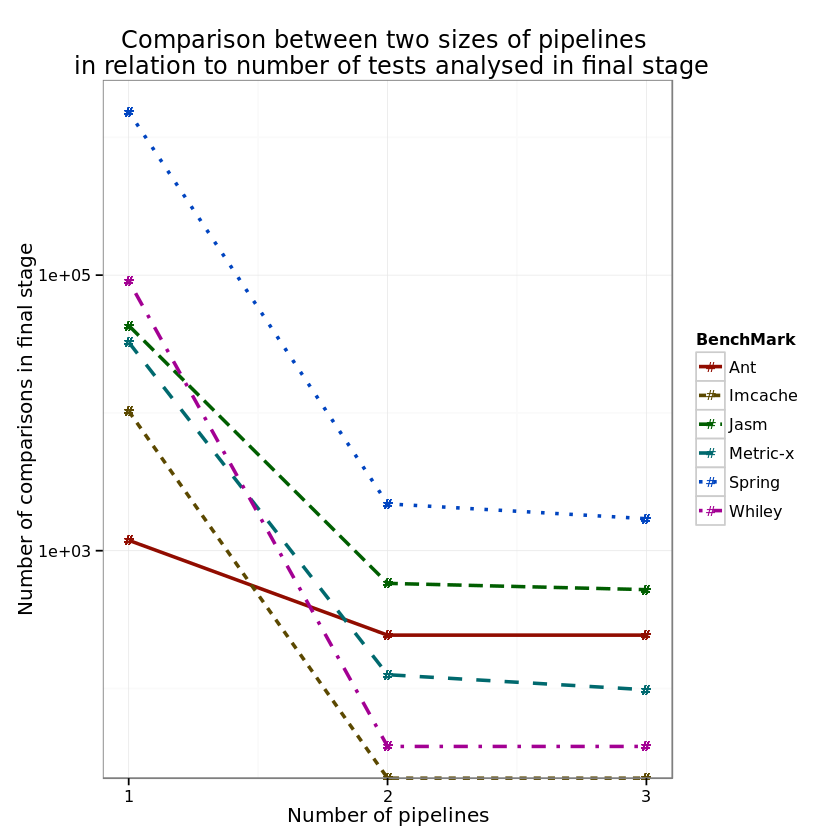
\includegraphics[height=10cm, width = 14.5cm]{Pipeline.png}
\end{center}
\caption{A figure showing the effect that using pipelines has on the number of comparisons that the final stage (Most computationally heavy) has to do.}
\label{fig:pipelinegraph}
\end{figure}

\subsection{Discussion}

The first hypothesis states an increase in the pipeline size will improve the factors of interest. The purpose of an increase in the pipeline size was to reduce the number of comparisons that the next stage had to perform. This reduction decreased the memory and time taken. Inspecting Figure \ref{fig:pipelinegraph}, it becomes clear that that pipeline size does improve the factors, but does not scale in every benchmark. Every two or three stage pipeline is a significant improvement on a single stage, however the majority of the benchmark's perform better with a two stage over a three. These results imply that the benchmarks that took less time using a two stage, were spending more time on the second stage than they were saving from the reduced number of comparisons in the third stage. 

Two situations which would cause more time to be spent on the second stage than was saved in the third stage are proposed. Firstly, each benchmark had it's own level of redundancy that was being looked for, this was dependent on how each benchmark reacted to different levels. Benchmarks with unit tests needed to have a higher level in comparison to benchmarks with end to end. Since each had their own percentage, this implies they also have their own optimal settings for the second pipeline. The settings were chosen by experimenting with different options, therefore a inefficient second pipeline would have contributed to the result.

The second reason is that there may be little difference between the outcome from the second and third pipelines. An example is shown in Figure \ref{fig:pipelinecomp}. Examining the three stage pipeline, it shows the first pipeline causes a large reduction in the number of comparisons needed implying that the tests are highly separable. Inserting the second stage, a limited amount of reduction occurs while being computationally heavy and passes the majority of test cases into the third and most computationally heavy stage. \todo{Talk about cost here.} This creates a situation where the number of identified redundant test cases has little change from stage two to three. This leads me to accept the first hypothesis, that increasing the pipeline size improves the factors of interest, however the optimal length is different for each benchmark.

The second hypothesis is that there is no difference between the number of output test cases. As expected, each benchmark had no significant change. If there were a change between the two pipelines with the same final stage settings could imply two things. Firstly, there is a bug in the code. Secondly, the second pipeline stage is more specific than the third. Since both pipelines of size two and three share the same settings in final stage, for the pipeline of size three, the second stage is a higher percentage than the final, this would cause a different output between the two sizes. 

\begin{figure}[h]
\centering
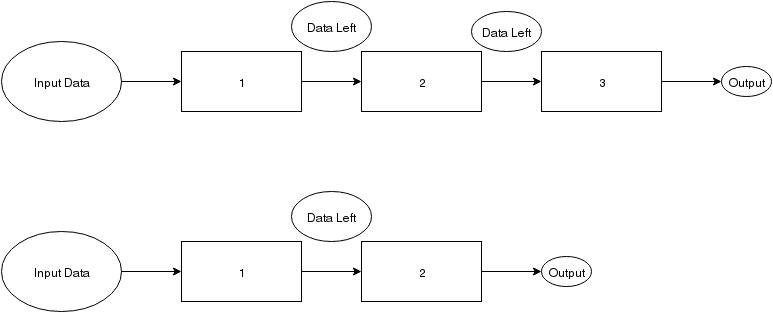
\includegraphics[width=\textwidth,height=8cm]{PipelineComp.png}
\caption{The circle size represents the data that is left in the pipeline. The figure shows that the difference that is between a two stage pipeline and a three stage only has limited room for a reduction in test cases identified. This shows that the time taken to run the extra pipeline costs more than it saves.}
\label{fig:pipelinecomp}
\end{figure}

\section{Experiment \rom{2} - K Depth Comparison}
\label{kdepthcomp}
\subsection{Motivation}
One of the abilities of the framework is to trace the K depth specified. This experiment is to determine the impact that altering the depth of K has on the overall cost. 

\begin{hyp}
The precision improvement from increasing K Depth outweighs the performance decrease.
\end{hyp}

\subsection{Settings}
There are three K depth's explored, one, two and three respectively.

\begin{itemize}
\item Difference between runs: K Depth
\end{itemize}

\subsection{Results}
Ant, Whiley and Spring appear to be the most responsive to the depth of K as shown in Figure \ref{fig:kdepthgraph} while the rest have limited change. Appendix \ref{fig:kdepthtime} shows the differences in time taken. Overall, for every benchmark there wasn't a large amount of change between them however it shows that as the K depth increases, the time taken increases.

\begin{figure}[h]
\begin{center}
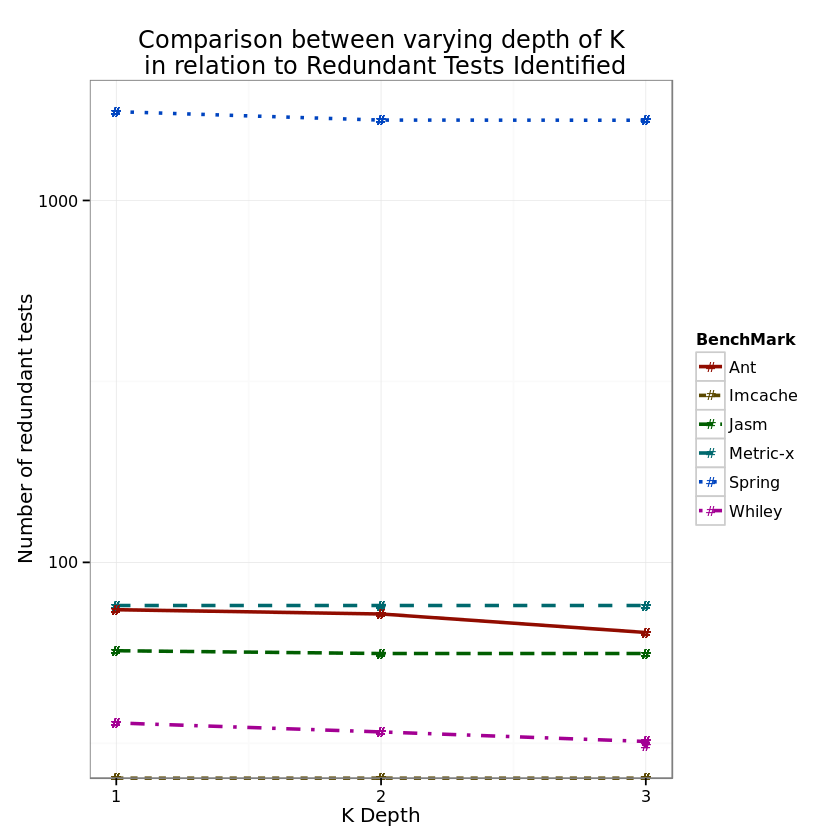
\includegraphics[height=10cm, width = 14.5cm]{KDepth.png}
\end{center}
\caption{A figure showing the effect that a change in the depth of the calling context has on the number of redundant tests are identified.}
\label{fig:kdepthgraph}
\end{figure}

\subsection{Discussion}
Increasing the depth of the calling context increases the amount of data that is analysed, intuitively making it more difficult for test cases to be the same. This should be reflected through a reduction in the overall tests identified. The extra data used is going cause extra analysis, this implies an increase in the time taken as calling context depth increases. It is expected that the precision increase is worth the performance decrease.

Examining Figure \ref{fig:kdepthgraph}, it shows that the number of redundant tests is only slightly decreased as the K depth increases. This shows several things. Firstly, it implies that when no other settings such as weighting or parameters are used, then the depth has limited effect on the redundant test cases identified. Secondly, the number of comparisons that were output from the first pipeline stage may cause there to be a limited differentiation. When the first pipeline stage outputs a low number of comparisons, then the final number of redundant tests identified would be similar regardless of the K depth specified, similar to the situation in Section \ref{sec:pipelineEva}. This occurs in Whiley, Metric-x, Imcache and Jasm. 

Increasing the depth of K has varying effect's on the time taken to analyse a benchmark. The differences are shown in Appendix \ref{fig:kdepthtime}. It shows that Ant, Imcache and Whiley have larger differences than the rest, however in the perspective of time these equate to around half a minute difference. Although increasing the depth has an smaller effect than expected on precision, the impact on time taken isn't substantial. Taking this into account, I can accept the hypothesis with the results implying that for some projects the calling context does not have to be particularly deep.

\section{Experiment \rom{3} - Parameter Comparison}
\label{sec:param}

\subsection{Motivation}
Parameters show the different contexts that a method was being called in. Retrieving this information gives us more confidence in determining whether two tests are redundant. The experiment explores the impact on performance and precision.

\begin{hyp}
Utilising parameters increases the time taken in comparison to a three stage pipeline.
\end{hyp}

\begin{hyp}
Utilising parameters increases the precision in comparison to a three stage pipeline.
\end{hyp}

\subsection{Settings}
The use of parameters is compared directly to the pipeline size three settings.

\begin{itemize}
\item Difference between runs: Parameters used during analysis
\end{itemize}

\subsection{Results}
The significant table for comparing parameters and no parameters is shown in Table \ref{parametersig}. It shows that there was a negative relation (increase) for every benchmark in regard to time taken. Every benchmark had a significantly positive effect (decrease) on the number of redundant test cases identified. This is not the case in Imcache due to it having zero redundant test cases identified in both, therefore no difference between the two.

\begin{table}[h]
\centering
\begin{tabular}{|l|l|l|}
\hline
{\bf }          & {\bf Total Time} & {\bf Redundant Tests Identified} \\ \hline
{\bf Whiley}    & +                & -                           \\ \hline
{\bf Jasm}      & +               & -                          \\ \hline
{\bf Ant}       & +                & -                           \\ \hline
{\bf Spring}    & +                & -                           \\ \hline
{\bf Imcache}   & +                & =                           \\ \hline
{\bf Metrics-x} & +                & -                           \\ \hline
\end{tabular}
\caption{A table showing the significant relationship between the use of parameters and no parameters for each benchmark}
\label{parametersig}
\end{table}

\begin{figure}[H]
\begin{center}
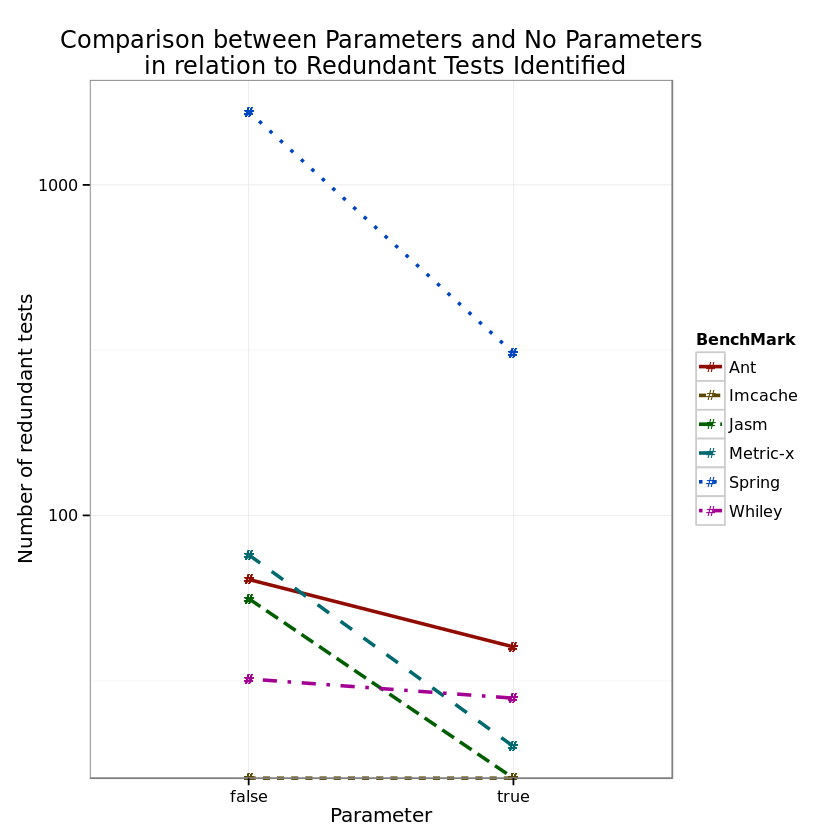
\includegraphics[height=10cm, width = 14.5cm]{Parameters.png}
\end{center}
\caption{A figure showing the effect that using parameters has on the number of redundant tests are identified.}
\label{fig:paramgraph}
\end{figure}

\subsection{Discussion}
Two factors have to be taken into account when discussing the impact of parameters on the time taken. Firstly, it is intuitive that analysing the extra data generated increases the time. The amount of increase is interesting, parameters only add extra computation when the method execution of the given K is exactly the same. For example, if test execution is $A ->  B ->  C$ is compared to $A ->  B ->  F$. Then the parameter won't be taken into account and therefore have limited effect on the time taken. 

The amount of time that the VM spends garbage collecting would also increase the time taken, due to increased amount of information in memory, the garbage collection process will have to execute more frequently for the analysis to continue to run. This would cause non-deterministic attributes to be increased. Examining Appendix \ref{fig:paramtime} -- Ant, Imcache, Jasm and Spring appear to affected by this due to the increased variance. This creates the hypothesises that parameters increase the precision and the total time taken. 

The significant Table \ref{fig:paramgraph} matches what is expected. For every benchmark, using parameters significantly increases the time taken. Examining Appendix \ref{fig:paramtime} shows how the benchmarks react with more detail. The most interesting would be Jasm. Without parameters, it analyses the data in less than one minute, with parameters, it takes just under five minutes. This may be indicative of the results discussed in Section \ref{kdepthcomp}. With K depth having little effect on a reduction in comparisons, the number of tests that match the K depth of three is higher than expected. This effect led to parameter information being examined more often, sequentially causing an increase in time taken. \todo{A factor that may have an accumulate effect} is related to the setup methods. If the set up methods are a large majority of the method calls, and match each other for the K depth, this would further increase the time taken. This allows us to accept hypothesis 4.

Every benchmark caused a significant decrease in the number of redundant test cases. Looking at Figure \ref{fig:paramgraph}, it confirms that every benchmark reacted with a substantial decrease in redundant tests identified, with Whiley being the least affected. This reiterates the discussion in Section \ref{kdepthcomp} that K depth is not enough of a factor to identify redundant test cases. It is expected that the number of false positives decrease, inspecting Table \ref{whileycoding} and \ref{metriccoding} gives insight into the types of tests identified. The Whiley benchmark coding shows that parameters remove the limited redundant tests as well as different array values. The Metric-x coding demonstrate a reduction in the number of the different parameter value tests identified substantially, from 52 to 8. Taking these coding tables into account, allow us to accept hypothesis 3.

\section{Experiment \rom{4} - Weighting Comparison}
\label{sec:weight}

\subsection{Motivation}
Utilising weighting is an attempt to remove any false positive tests identified. The experiment attempts to identify if weighting has any potential to remove these false positives, while exploring the impact on performance.

\begin{hyp}
Weighting decreases the number of false positives compared to a standard three stage pipeline
\end{hyp}

\begin{hyp}
Weighting decreases the time taken compared to a standard three stage pipeline
\end{hyp}

\subsection{Settings}
The use of weighting is compared directly to the pipeline size three settings.

\begin{itemize}
\item Difference between runs: Weighting Used
\end{itemize}

\subsection{Results}
The significant table for comparing the use of weighting is shown in Table \ref{weightingsig}. There are a mixture of results in regard to the total time taken -- Whiley, Ant and Imcache had a significantly negative relation and weighting increased the time taken to analyse. Jasm, Spring and Metric-x had a significantly positive relation and weighting decreased the time taken to analyse. The majority -- Whiley, Ant, Jasm and Metrics-x had a significantly positive relation in regard to the number of redundant tests identified, showing a decrease in the number identified when weighting was applied. Spring was the only benchmark where weighting had a significantly negative impact.

\begin{table}[h]
\centering


\begin{tabular}{|l|l|l|}
\hline
{\bf }          & {\bf Total Time} & {\bf Redundant Tests Identified} \\ \hline
{\bf Whiley}    & +                & -                           \\ \hline
{\bf Jasm}      & -                & -                           \\ \hline
{\bf Ant}       & +                & -                           \\ \hline
{\bf Spring}    & -                & +                           \\ \hline
{\bf Imcache}   & +                & =                           \\ \hline
{\bf Metrics-x} & -                & -                           \\ \hline
\end{tabular}
\caption{A table showing the significant relationship between the use of weighting and no weighting for each benchmark}
\label{weightingsig}
\end{table}


\begin{figure}[h]
\begin{center}
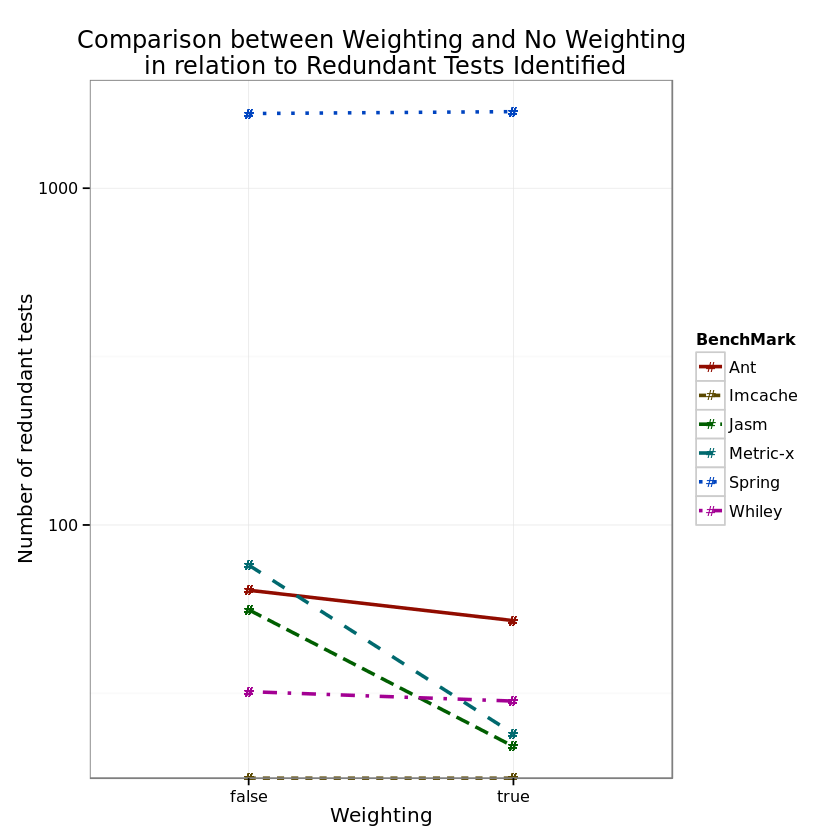
\includegraphics[height=10cm, width = 14.5cm]{Weighting.png}
\end{center}
\caption{A figure showing the effect that using weighting has on the number of redundant tests are identified.}
\label{fig:weightgraph}
\end{figure}

\subsection{Discussion}
As previously discussed in Section \ref{C:related}, much of the related work encountered difficulties with test cases sharing setup and teardown method calls, resulting in a high false positive rate. Intuitively this makes sense when the test cases are small in comparison to the setup and teardown methods where the setup and teardown methods represent a large majority of the test data. The approach of removing a portion of the most executed method calls meant that the amount of data that would be compared decreases. This should reflect onto the results by showing a decrease in the time taken, as per hypothesis 7. The effect that it has on the number of redundant test cases should be dependent on the benchmark when weighting is used. This is because removing the most common tests should imply an decreased false-positive rate, but also may increase the number of actual redundant tests picked up. The precision is of interest when examining the cause effect of weighting, this is reflected by hypothesis 6.

Table \ref{weightingsig} shows a mixture of results in regard to the total time taken. Two out of the three benchmarks that had a significant increase in the total time were small benchmarks. This may imply that the size of the benchmark has some relation to the effect of weighting on the time taken. One reason is that weighting is calculated once per test case per analysis stage. The weighting calculation has a linear relation with the number of test cases. In comparison, every test case is compared to every other, therefore a factorial relation with the number of test cases. Since the factorial relation is closer to linear, the smaller the number of redundant test cases. Then the smaller the number, the more impact the linear weight calculation has on the overall time taken. This may explain a relation between size and time taken. Examining the overall impact from weighting on the time taken in Appendix \ref{fig:weighttime} allows us to invalidate hypothesis 7 as there is no general consensus between benchmarks.

A reduction in the false positive rate was weightings primary goal. Spring was the only benchmark that significantly increased the number of redundant test cases identified. The other benchmarks had a significant decrease. At first, this makes it appear that by using weighting it may solve some of the issues that were identified in \cite{koochakzadeh2009test} \cite{li2008static}. To confirm this, examining Table \ref{whileycoding} and \ref{metriccoding} will give insight into the effect of weighting. Comparing the two columns for the Whiley coding, Pipeline 2 and Weighting, the only difference is the removal of the two limited redundancy test cases that were picked up by Pipeline 2. The weighting is able to remove the test cases that have similar set up and tear down methods, but fails to reduce the number of other redundancies. By removing the method executions that were common throughout the benchmarks, this led to a decrease in false positive tests identified. The Metric-x coding paints a similar story. Weighting reduces the number of parameter value redundancies identified as well as the limited redundancies, however does not completely remove them. This is interesting and implies that the number of setup and tear down methods that remained in the data analysed was still a large portion of the data. We are able to accept hypothesis 6, although work remains to improve the weighting method to remove redundant tests completely.


\section{Experiment \rom{5} - Weighting and Parameter Comparison}

\subsection{Motivation}
Combining weighting and parameters is an attempt to reduce the number of false positives, and at the same time increase the confidence that the redundant tests are truly redundant. 

\begin{hyp}
A combination of weighting and parameters increases the precision in comparison to weighting and parameters separately
\end{hyp}

\subsection{Settings}
There are several comparisons that occur in this experiment. The use of weighting with parameters is compared directly to both, the pipeline size two settings as well as weighting and parameters separately.

\begin{itemize}
\item Difference between runs: Weighting and Parameters combined
\end{itemize}

\subsection{Results}
The relevant significance table is shown in Table \ref{weightingparamsig}, it shows a comparison between the combination of techniques and pipeline of size two. It shows that for every Benchmark apart from Imcache, there was a negative relation for the time taken, indicating that the time increased when using weighting and parameters for the majority of benchmarks. In contrast to this, every benchmark had a positive relation to the number of redundant tests identified. Figure \ref{fig:weightingparamgraph} indicates the number of tests identified for each benchmark in comparison to weighting and parameters separately. Each benchmark reacted differently to the use of weighting and parameters combined -- Spring, Jasm and Metric-x had large decreases compared to the weighting with the rest being similar between the three types. 

\begin{table}[h]
\centering

\begin{tabular}{|l|l|l|}
\hline
{\bf }          & {\bf Total Time} & {\bf Redundant Tests Identified} \\ \hline
{\bf Whiley}    & +                & -                           \\ \hline
{\bf Jasm}      & +                & -                           \\ \hline
{\bf Ant}       & +                & -                           \\ \hline
{\bf Spring}    & +                & -                           \\ \hline
{\bf Imcache}   & -                & =                           \\ \hline
{\bf Metrics-x} & +                & -                           \\ \hline
\end{tabular}
\caption{A table showing the significant relationship between the use of weighting with parameters and pipeline size two for each benchmark}
\label{weightingparamsig}
\end{table}

\begin{figure}[h]
\begin{center}
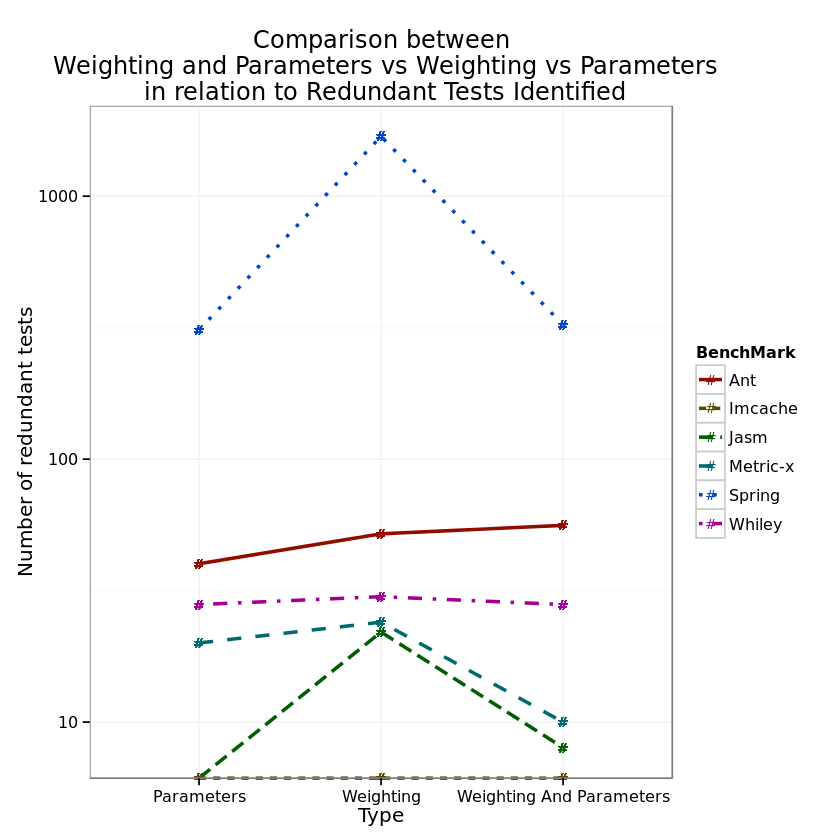
\includegraphics[height=10cm, width = 14.5cm]{WeightNParamVAll.png}
\end{center}
\caption{A figure showing the effect that using weighting and parameters has on the number of redundant tests are identified.}
\label{fig:weightingparamgraph}
\end{figure}

\subsection{Discussion}
Using parameters to increase the confidence, and weighting to remove common method executions should increase the precision of the framework. To appraise the combination, Figure \ref{fig:weightingparamgraph} displays the comparison between each of the three techniques. Weighting identified more redundant tests in every benchmark except Ant. Parameters produce similar results to the combination, apart from in Jasm and Metric-x. Whiley coding in Table \ref{whileycoding} show no difference between parameters and the combination. Metric-x's coding Table \ref{metriccoding} hints that the combination may have some appeal by removing all eight limited redundancy tests. At the same time, the similar tests are also removed which is a negative outcome. This suggests that the combination improves the precision for some benchmarks, but not for others. This conclusion means hypothesis 8 can not be accepted. 

Combining weighting and parameters presents interesting time taken results. Table \ref{weightingparamsig} shows that it is nearly identical to the parameters significance table with the only exception being that the Imcache benchmark changed from significant increase in time to a significant decrease in time. This indicates that parameters have a stronger effect than weighting on the final outcome. This is an unexpected result. As previously discussed in Section \ref{sec:param}, one of the reasons that parameters increase the time taken is due to the similar setup and tear down method calls. With weighting removing a large portion of the common method executions it would be expected to cause a decrease in the number of comparisons using parameters. Looking at Appendix \ref{fig:weightparamvparamtime}, this appears to be true for Jasm, Metric-x, Spring and Imcache. However, for Whiley and Ant benchmarks the time to calculate the weighting information is taking longer than the comparisons saved. 

\section{Redundant Test Case Coding}

\begin{table}[h]
\centering

\begin{tabular}{|l|l|l|l|l|}
\hline
                          & \multicolumn{4}{c|}{{\bf Whiley}}                                                             \\ \hline
{\bf Types of redundancy} & \multicolumn{1}{c|}{{\bf Pipeline 2}} & {\bf Weighting} & {\bf Parameters} & {\bf Parameters and Weighting} \\ \hline
Different Equation Value  & 6                                     & 6               & 6                & 6                \\ \hline
Different Equation Sign   & 8                                     & 8               & 8                & 8                \\ \hline
Different Array Values    & 2                                     & 2               & 0                & 0                \\ \hline
Same                      & 10                                    & 10              & 10               & 10               \\ \hline
Limited Redundancy        & 2                                     & 0               & 0                & 0                \\ \hline
Rearranged Equation       & 2                                     & 2               & 2                & 2                \\ \hline
Extra if statement        & 2                                     & 2               & 2                & 2                \\ \hline
                          &                                       &                 &                  &                  \\ \hline
{\bf Total}               & 32                                    & 30              & 28               & 28               \\ \hline
\end{tabular}
\caption{A table displaying a list of coding's for the Whiley Benchmark for four of the different techniques used.}
\label{whileycoding}
\end{table}


\begin{table}[]
\centering
\begin{tabular}{|l|l|l|l|l|}
\hline
                             & \multicolumn{4}{c|}{\textbf{Metric-X}}                                                              \\ \hline
\textbf{Types of redundancy} & \textbf{Pipeline 2} & \textbf{Weighting} & \textbf{Parameters} & \textbf{Parameters  And Weighting} \\ \hline
Different Parameter Value    & 52                  & 10                 & 8                   & 4                                  \\ \hline
Different Object Type        & 6                   & 2                  & 2                   & 0                                  \\ \hline
Different Array Values       & 8                   & 6                  & 4                   & 6                                  \\ \hline
Similar                      & 2                   & 2                  & 0                   & 0                                  \\ \hline
Limited Redundancy           & 8                   & 4                  & 6                   & 0                                  \\ \hline
\textbf{}                    &                     &                    &                     &                                    \\ \hline
\textbf{Total}               & 76                  & 24                 & 20                  & 10                                 \\ \hline
\end{tabular}
\caption{A table displaying a list of coding's for the Whiley Benchmark for four of the different techniques used.}
\label{metriccoding}
\end{table}
